%&pdflatex
\documentclass{standalone}
\usepackage{tikz}
\usetikzlibrary{arrows}
\usetikzlibrary{shapes}

\begin{document}

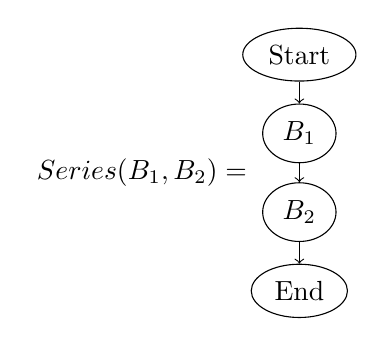
\begin{tikzpicture}
    \node (Sc) at (1,1.5) { \(Series(B_1,B_2)=\)};
    \node[draw, ellipse] (S) at (3,3) {Start};
    \node[draw, ellipse] (B1) at (3, 2) {\( B_1 \)};
    \node[draw, ellipse] (B2) at (3, 1) {\( B_2 \)};
    \node[draw, ellipse] (T) at (3, 0) {End};

    \draw[->] (S) to (B1);
    \draw[->] (B1) to (B2);
    \draw[->] (B2) to (T);
\end{tikzpicture}

\end{document}



